% $Id: gmmdip.tex,v 1.23 2008/04/16 17:10:30 Moritz.Ringler Exp $
%
%
\section{GMM-DIP -- generalized Mie scattering of a dipole field}\label{app.gmmdip}\index{GMM-DIP}
Both GMM and GMM-FIELD use a plane wave as the incident light field. To describe
the emission of a dye molecule or an atom as in
\cite{phdrin08, rin08} the plane wave must be exchanged against that
of an oscillating dipole. The program thus obtained is called
GMM-DIP%
\footnote{The source code of GMM-FIELD  as well as some example applications
can be downloaded from
\mbox{\uri{http://moritz-ringler.name/dissertation/GMM\_DIP.tar.bz2}}.}.
GMM-DIP also differs from GMM in the output quantities:
cross sections make little sense for a dipole field and their place is taken
by the absorbed and radiated powers
$P_\mathrm{abs}/P_0$ and $P_\mathrm{r}/P_0$.

The oscillating dipole is treated like an additional particle throughout
most of the program. A 'particle index' of zero would be a canonical choice
but for practical reasons the dipole simply gets the index
$\beta = N + 1$ where $N$ is the number of scatterers.

In this fashion we arrive at the program structure for GMM-DIP that is represented
in figure~\ref{abb.gmmdip}. Changes with respect to GMM-FIELD are
highlighted in blue. The way the powers
$P_\mathrm{r}$ and $P_\mathrm{abs}$ are calculated is described in
\cite{rin08, phdrin08}. It is quite
similar to the way the cross sections are calculated in the original GMM.
In the routine that calculates the near field the initialization of
$\evec$ is changed: instead of  $\evec = \exp{i k z}\,\ex$
we now use
$\evec = \vec{0}$, the incident field is
evaluated in the same way as the scattered field of the particles.

\begin{algorithm}[ht]
\KwData{$n_\mathrm{max}$, $\lambda$, $N$; $\vec{r}^\beta$, $\vec{r}^{\mathrm{Dipol}}$, $R^\beta$, $\epsint^\beta$}
\KwResult{$g_\mathrm{r}=P_\mathrm{r}/P_0$, $g_\mathrm{ET}=P_\mathrm{abs}/P_0$}
\Begin{
read wavelength\;
read aggregate parameters\;
calculate Mie coefficients for all spheres\;
{\color{darkblue} $\beta_\mathrm{max} = N + 1$\;}
calculate vector translation coefficients\;{\color{darkblue}
\tcp{expansion of the dipole field in vector spherical harmonics}
$a^{N + 1}_{1\,1} = -i/\sqrt{3}$\;
$a^{N + 1}_{-1\,1} = i/\sqrt{3}$\;
calculate the vector translation of the dipole fields $\rightarrow p_{mn}^{0\;\beta},\ q_{mn}^{0\;\beta}$\;
$\beta_\mathrm{max} = N$\;
}
calculate scattering coefficientsn $\rightarrow a_{mn}^\beta, b_{mn}^\beta$\;
{\color{darkblue}
$\beta_\mathrm{max} = N + 1$\;
\tcp{if you want just the scattered field}
\tcp{$\beta_\mathrm{max} = N$}
}
calculate and write the near field\;
{\color{darkblue}
$\beta_\mathrm{max} = N + 1$\;
calculate $g_\mathrm{r} = P_\mathrm{r}/P_0$\;
$\beta_\mathrm{max} = N$\;
calculate $P_\mathrm{str}/P_0$\;
calculate $P_\mathrm{ext}/P_0$\;
$g_\mathrm{ET} = P_\mathrm{ext}/P_0 -  P_\mathrm{str}/P_0$\;
write $g_\mathrm{r}$ and $g_\mathrm{ET}$\;
}
}
\caption{Program structure of GMM-DIP.}\label{abb.gmmdip}
\end{algorithm}

The coordinates of the dipole that models the emitting atom or
molecule are specified in the input file defining the field and the
aggregate geometry as if it was another particle. Though the dipole
has neither radius nor refractive index both must be entered.
The value of the refractive index is not used by the program, the
'dipole radius' determines the size of the volume around the dipole
in which the field is not evaluated.

As an example, we show here the field and aggregate definition file
for a dipole that is located in the middle between two
gold particles with radius $R = \val{20}{nm}$ and
surface-to-surface distance $\dss = \val{20}{nm}$. The dipole emits at
$\lambda = \val{532}{nm}$. The whole arrangement
is immersed in water.
\begin{verbatim}
0.39886 = wavelength (vacuum wavelength: 0.532)
3 = #spheres + 1 (dipole); <= nLp in gmm01f.par
 0.03 0 0 0.02000 0.417515 1.66004 = x, y, z, r, Re(n), Im(n)
-0.03 0 0 0.02000 0.417515 1.66004 = x, y, z, r, Re(n), Im(n)
 0.00 0 0 0.00001 1.000000 0.00000 = x, y, z, (r, Re(n), Im(n)) <- dipole
\end{verbatim}
Again, we have used microns as the length unit.
The position of the dipole at the center of the coordinate system
(that is not a necessity -- it can be anywhere) is set in the last line.
The dipole orientation is always parallel to the $x$-axis, and therefore
in this case also parallel to the dimer axis. The embedding medium
is taken into account by specifying the in-water wavelength
$\lambda = \lambda_0 / \sqrt{\epsi{H2O}}$ and
by specifying the complex refractive index of the particles $\sqrt{\epsi{Au}}$
in units of the (purely real) refractive index of the medium
$\sqrt{\epsi{H2O}}$.

\subsection{Comparison with published MMP results on fluorescence
quenching near a single particle}

\begin{figure}
\begin{center}
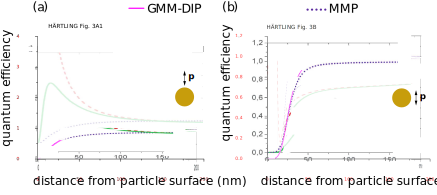
\includegraphics[width=0.8\textwidth]{abb/gmmdiphaert}
\caption[GMM-DIP, comparison with MMP results for a single particle]{
\textbf{GMM-DIP, quantitative comparison with MMP
 results for a single particle.}
 quantum efficiency for a dipole that is oriented (a) radially and (b)
 tangentially with respect to a nearby gold nanoparticle. The dipole
 has intrinsic quantum efficiency one, the particle is the same as that
in \reffig{abb.gmmhaertb}.  The MMP results from \cite{hae07}
are dotted in violet, the GMM-DIP results are shown as a magenta-colored
solid line.  The red and green lines are H�rtling's results
on the excitation enhancement and on the total enhancement and
can be ignored at this point (see also \reffig{abb.gmmhaerta}).
}\label{abb.gmmdiphaert}
\end{center}
\end{figure}

We have reproduced the MMP results on fluorescence quenching near
a single gold particle published by H�rtling et al. in \cite{hae07}
as a test of GMM-DIP. We consider the quantum efficiency of a dipole emitter
near a single gold particle with a diameter of \val{80}{nm} that emits at
$\lambda=\val{560}{nm}$ with an intrinsic quantum efficiency of one.
The surrounding medium has refractive index one. The quantum efficiency of the
quenched dipole is calculated from the Purcell factor $g_\mathrm{r}=P_\mathrm{r}/P_0$
and the energy transfer factor $g_\mathrm{ET}=P_\mathrm{abs}/P_0$ as %
\footnote{Note that the monochromatic dipole model used here is not sufficient
to describe a multi-level dye molecule. See \cite{rin08} for details.}
\begin{equation}
\eta = \frac{g_\mathrm{r}}{g_\mathrm{r} + g_\mathrm{ET}}
\end{equation}
Again we consider the two most important geometric arrangements, namely
a dipole with parallel and perpendicular orientation with respect to the
nanoparticle surface. The geometries and the results are shown in
\reffig{abb.gmmdiphaert}. GMM-DIP and MMP results agree almost perfectly.

\subsection{Feedback -
Comparison with results on fluorescence
quenching near a single particle in the Gersten-Nitzan model}
We will now compare GMM-DIP results for the Purcell factor $g_\mathrm{r}$
and the energy transfer factor $g_\mathrm{ET}$ of a dipole near a single
gold nanoparticle with the results for the same quantities
obtained with the Gersten-Nitzan model \cite{ger81}.
Apart from the fact that the Gersten-Nitzan model cannot be applied to
aggregates, it differs from GMM-DIP in two important aspects.
First, it uses a quasistatic approximation whereas GMM-DIP is fully retarded,
second, it takes into account re-excitation of the emitter by its own field
scattered by the nanoparticle. We call this phenomenon feedback.

Again, we use an example to compare the two models. We consider the
model system of \cite{dul05}: a dipole that emits at $\lambda=\val{668}{nm}$
near a nanoparticle with a diameter of \val{16}{nm} immersed in water.
Gersten-Nitzan data are calculated with ETCALC\index{ETCALC}\footnote{%
ETCALC is a C implementation of the Gersten-Nitzan model developed in our group
in Munich. The source code is available at
\mbox{\uri{http://moritz-ringler.name/dissertation/ETCALC.tar.bz2}}.
Feedback can be switched on and off by means of the compile
time parameter \texttt{GN\_FEEDBACK} in the header file
etcalc.h.}. We vary the distance between particle and dipole.
Fig.~\ref{abb.gmmdipgn} shows the Purcell
factor and the energy transfer factor for radial and tangential dipole orientation.

\begin{figure}
\begin{center}
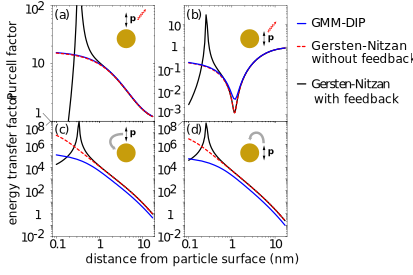
\includegraphics{abb/gmmdipgn}
\caption{
\textbf{GMM-DIP,
quantitative comparison with Gersten-Nitzan results for a single particle.}
Purcell factor (a,b) und energy transfer factor (c,d)
for a monochromatic dipole near a single gold nanoparticle; calculated with
GMM-DIP, the Gersten-Nitzan model without feedback and the
Gersten-Nitzan model with feedback.
\textbf{(a)~and (c)~radial orientation.}
\textbf{(b)~and (d)~tangential orientation.}
}\label{abb.gmmdipgn}
\end{center}
\end{figure}

Let us first have a look at the effect of feedback. This effect
becomes significant only at distances of less than \val{1}{nm} and large only at
distances of less than ca. \val{0.5}{nm}. At these distances, non-local
interactions \cite{leu90} and charge transfer \cite{dex53} cannot be neglected
any more. A distance of \val{0.5}{nm} is also comparable
to the typical size of a dye molecule. It is a rather gross approximation
to model a dye molecule with a point dipole in this situation.
Therefore, the accuracy both of the Mie-theoretical prediction and of the
Gersten-Nitzan prediction concerning the nanoparticle-induced change of the
rates is limited in this distance range. Instead, at least the molecule should
be treated quantum-mechanically. This will in general only be possible with
purely numerical methods \cite{and04}.

We now compare GMM-DIP and Gersten-Nitzan without feedback. In the
Purcell factor,
GMM-DIP and Gersten-Nitzan without feedback agree almost perfectly
(\reffig{abb.gmmdipgn}a and~b). Only the suppression of emission
for the tangential orientation at distances of about
\val{1}{nm} is more pronounced in the Gersten-Nitzan model.
The absolute difference between the GMM-DIP result and the Gersten-Nitzan
result is small and can have numerical causes or be due to small differences
in the dielectric function used.

The Gersten-Nitzan model predicts an energy transfer rate that is larger
by a factor of about two than
that predicted by the Mie-type calculation
for distances larger than about \val{1}{nm} (\reffig{abb.gmmdipgn}c and~d).
The GMM-DIP results agree with the independent MMP calculations of
\cite{hae07} as we have seen in \reffig{abb.gmmdiphaert}. Therefore, the
cause of this discrepancy is more likely to be found in the Gersten-Nitzan model
and in its implementation than in GMM-DIP.

For distances of less than about \val{0.5}{nm} the discrepancy between
Gersten-Nitzan and GMM-DIP becomes larger. This might be due to the fact that
higher order multipoles are neglected in the Gersten-Nitzan model.

In summary, we can say that the Mie-theoretical description
implemented in GMM-DIP and the Gersten-Nitzan description implemented in ETCALC
agree quantitatively in the Purcell factor and qualitatively in the energy
transfer factor if feedback is not taken into account. The effect of feedback
becomes large only at distances of less than about half a nanometer where the
assumptions underlying both models start to become less and less valid anyways.
